\documentclass[1p]{elsarticle_modified}
%\bibliographystyle{elsarticle-num}

%\usepackage[colorlinks]{hyperref}
%\usepackage{abbrmath_seonhwa} %\Abb, \Ascr, \Acal ,\Abf, \Afrak
\usepackage{amsfonts}
\usepackage{amssymb}
\usepackage{amsmath}
\usepackage{amsthm}
\usepackage{scalefnt}
\usepackage{amsbsy}
\usepackage{kotex}
\usepackage{caption}
\usepackage{subfig}
\usepackage{color}
\usepackage{graphicx}
\usepackage{xcolor} %% white, black, red, green, blue, cyan, magenta, yellow
\usepackage{float}
\usepackage{setspace}
\usepackage{hyperref}

\usepackage{tikz}
\usetikzlibrary{arrows}

\usepackage{multirow}
\usepackage{array} % fixed length table
\usepackage{hhline}

%%%%%%%%%%%%%%%%%%%%%
\makeatletter
\renewcommand*\env@matrix[1][\arraystretch]{%
	\edef\arraystretch{#1}%
	\hskip -\arraycolsep
	\let\@ifnextchar\new@ifnextchar
	\array{*\c@MaxMatrixCols c}}
\makeatother %https://tex.stackexchange.com/questions/14071/how-can-i-increase-the-line-spacing-in-a-matrix
%%%%%%%%%%%%%%%

\usepackage[normalem]{ulem}

\newcommand{\msout}[1]{\ifmmode\text{\sout{\ensuremath{#1}}}\else\sout{#1}\fi}
%SOURCE: \msout is \stkout macro in https://tex.stackexchange.com/questions/20609/strikeout-in-math-mode

\newcommand{\cancel}[1]{
	\ifmmode
	{\color{red}\msout{#1}}
	\else
	{\color{red}\sout{#1}}
	\fi
}

\newcommand{\add}[1]{
	{\color{blue}\uwave{#1}}
}

\newcommand{\replace}[2]{
	\ifmmode
	{\color{red}\msout{#1}}{\color{blue}\uwave{#2}}
	\else
	{\color{red}\sout{#1}}{\color{blue}\uwave{#2}}
	\fi
}

\newcommand{\Sol}{\mathcal{S}} %segment
\newcommand{\D}{D} %diagram
\newcommand{\A}{\mathcal{A}} %arc


%%%%%%%%%%%%%%%%%%%%%%%%%%%%%5 test

\def\sl{\operatorname{\textup{SL}}(2,\Cbb)}
\def\psl{\operatorname{\textup{PSL}}(2,\Cbb)}
\def\quan{\mkern 1mu \triangleright \mkern 1mu}

\theoremstyle{definition}
\newtheorem{thm}{Theorem}[section]
\newtheorem{prop}[thm]{Proposition}
\newtheorem{lem}[thm]{Lemma}
\newtheorem{ques}[thm]{Question}
\newtheorem{cor}[thm]{Corollary}
\newtheorem{defn}[thm]{Definition}
\newtheorem{exam}[thm]{Example}
\newtheorem{rmk}[thm]{Remark}
\newtheorem{alg}[thm]{Algorithm}

\newcommand{\I}{\sqrt{-1}}
\begin{document}

%\begin{frontmatter}
%
%\title{Boundary parabolic representations of knots up to 8 crossings}
%
%%% Group authors per affiliation:
%\author{Yunhi Cho} 
%\address{Department of Mathematics, University of Seoul, Seoul, Korea}
%\ead{yhcho@uos.ac.kr}
%
%
%\author{Seonhwa Kim} %\fnref{s_kim}}
%\address{Center for Geometry and Physics, Institute for Basic Science, Pohang, 37673, Korea}
%\ead{ryeona17@ibs.re.kr}
%
%\author{Hyuk Kim}
%\address{Department of Mathematical Sciences, Seoul National University, Seoul 08826, Korea}
%\ead{hyukkim@snu.ac.kr}
%
%\author{Seokbeom Yoon}
%\address{Department of Mathematical Sciences, Seoul National University, Seoul, 08826,  Korea}
%\ead{sbyoon15@snu.ac.kr}
%
%\begin{abstract}
%We find all boundary parabolic representation of knots up to 8 crossings.
%
%\end{abstract}
%\begin{keyword}
%    \MSC[2010] 57M25 
%\end{keyword}
%
%\end{frontmatter}

%\linenumbers
%\tableofcontents
%
\newcommand\colored[1]{\textcolor{white}{\rule[-0.35ex]{0.8em}{1.4ex}}\kern-0.8em\color{red} #1}%
%\newcommand\colored[1]{\textcolor{white}{ #1}\kern-2.17ex	\textcolor{white}{ #1}\kern-1.81ex	\textcolor{white}{ #1}\kern-2.15ex\color{red}#1	}

{\Large $\underline{11a_{79}~(K11a_{79})}$}

\setlength{\tabcolsep}{10pt}
\renewcommand{\arraystretch}{1.6}
\vspace{1cm}\begin{tabular}{m{100pt}>{\centering\arraybackslash}m{274pt}}
\multirow{5}{120pt}{
	\centering
	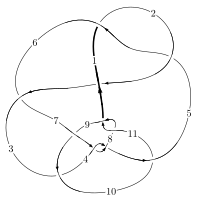
\includegraphics[width=112pt]{../../../GIT/diagram.site/Diagrams/png/328_11a_79.png}\\
\ \ \ A knot diagram\footnotemark}&
\allowdisplaybreaks
\textbf{Linearized knot diagam} \\
\cline{2-2}
 &
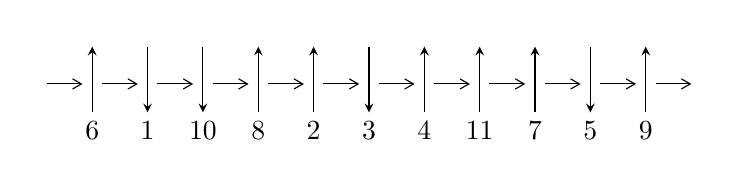
\begin{tikzpicture}[x=20pt, y=17pt]
	% nodes
	\node (C0) at (0, 0) {};
	\node (C1) at (1, 0) {};
	\node (C1U) at (1, +1) {};
	\node (C1D) at (1, -1) {6};

	\node (C2) at (2, 0) {};
	\node (C2U) at (2, +1) {};
	\node (C2D) at (2, -1) {1};

	\node (C3) at (3, 0) {};
	\node (C3U) at (3, +1) {};
	\node (C3D) at (3, -1) {10};

	\node (C4) at (4, 0) {};
	\node (C4U) at (4, +1) {};
	\node (C4D) at (4, -1) {8};

	\node (C5) at (5, 0) {};
	\node (C5U) at (5, +1) {};
	\node (C5D) at (5, -1) {2};

	\node (C6) at (6, 0) {};
	\node (C6U) at (6, +1) {};
	\node (C6D) at (6, -1) {3};

	\node (C7) at (7, 0) {};
	\node (C7U) at (7, +1) {};
	\node (C7D) at (7, -1) {4};

	\node (C8) at (8, 0) {};
	\node (C8U) at (8, +1) {};
	\node (C8D) at (8, -1) {11};

	\node (C9) at (9, 0) {};
	\node (C9U) at (9, +1) {};
	\node (C9D) at (9, -1) {7};

	\node (C10) at (10, 0) {};
	\node (C10U) at (10, +1) {};
	\node (C10D) at (10, -1) {5};

	\node (C11) at (11, 0) {};
	\node (C11U) at (11, +1) {};
	\node (C11D) at (11, -1) {9};
	\node (C12) at (12, 0) {};

	% arrows
	\draw[->,>={angle 60}]
	(C0) edge (C1) (C1) edge (C2) (C2) edge (C3) (C3) edge (C4) (C4) edge (C5) (C5) edge (C6) (C6) edge (C7) (C7) edge (C8) (C8) edge (C9) (C9) edge (C10) (C10) edge (C11) (C11) edge (C12) ;	\draw[->,>=stealth]
	(C1D) edge (C1U) (C2U) edge (C2D) (C3U) edge (C3D) (C4D) edge (C4U) (C5D) edge (C5U) (C6U) edge (C6D) (C7D) edge (C7U) (C8D) edge (C8U) (C9D) edge (C9U) (C10U) edge (C10D) (C11D) edge (C11U) ;
	\end{tikzpicture} \\
\hhline{~~} \\& 
\textbf{Solving Sequence} \\ \cline{2-2} 
 &
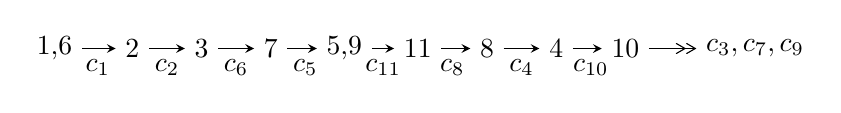
\begin{tikzpicture}[x=25pt, y=7pt]
	% node
	\node (A0) at (-1/8, 0) {1,6};
	\node (A1) at (1, 0) {2};
	\node (A2) at (2, 0) {3};
	\node (A3) at (3, 0) {7};
	\node (A4) at (65/16, 0) {5,9};
	\node (A5) at (41/8, 0) {11};
	\node (A6) at (49/8, 0) {8};
	\node (A7) at (57/8, 0) {4};
	\node (A8) at (65/8, 0) {10};
	\node (C1) at (1/2, -1) {$c_{1}$};
	\node (C2) at (3/2, -1) {$c_{2}$};
	\node (C3) at (5/2, -1) {$c_{6}$};
	\node (C4) at (7/2, -1) {$c_{5}$};
	\node (C5) at (37/8, -1) {$c_{11}$};
	\node (C6) at (45/8, -1) {$c_{8}$};
	\node (C7) at (53/8, -1) {$c_{4}$};
	\node (C8) at (61/8, -1) {$c_{10}$};
	\node (A9) at (10, 0) {$c_{3},c_{7},c_{9}$};

	% edge
	\draw[->,>=stealth]	
	(A0) edge (A1) (A1) edge (A2) (A2) edge (A3) (A3) edge (A4) (A4) edge (A5) (A5) edge (A6) (A6) edge (A7) (A7) edge (A8) ;
	\draw[->>,>={angle 60}]	
	(A8) edge (A9);
\end{tikzpicture} \\ 

\end{tabular} \\

\footnotetext{
The image of knot diagram is generated by the software ``\textbf{Draw programme}" developed by Andrew Bartholomew(\url{http://www.layer8.co.uk/maths/draw/index.htm\#Running-draw}), where we modified some parts for our purpose(\url{https://github.com/CATsTAILs/LinksPainter}).
}\phantom \\ \newline 
\centering \textbf{Ideals for irreducible components\footnotemark of $X_{\text{par}}$} 
 
\begin{align*}
I^u_{1}&=\langle 
-1.23376\times10^{38} u^{70}-2.60156\times10^{38} u^{69}+\cdots+3.74973\times10^{38} b-3.48298\times10^{38},\\
\phantom{I^u_{1}}&\phantom{= \langle  }6.34585\times10^{38} u^{70}+1.49012\times10^{39} u^{69}+\cdots+3.74973\times10^{38} a-1.05045\times10^{39},\;u^{71}+3 u^{70}+\cdots-2 u-1\rangle \\
\\
\end{align*}
\raggedright * 1 irreducible components of $\dim_{\mathbb{C}}=0$, with total 71 representations.\\
\footnotetext{All coefficients of polynomials are rational numbers. But the coefficients are sometimes approximated in decimal forms when there is not enough margin.}
\newpage
\renewcommand{\arraystretch}{1}
\centering \section*{I. $I^u_{1}= \langle -1.23\times10^{38} u^{70}-2.60\times10^{38} u^{69}+\cdots+3.75\times10^{38} b-3.48\times10^{38},\;6.35\times10^{38} u^{70}+1.49\times10^{39} u^{69}+\cdots+3.75\times10^{38} a-1.05\times10^{39},\;u^{71}+3 u^{70}+\cdots-2 u-1 \rangle$}
\flushleft \textbf{(i) Arc colorings}\\
\begin{tabular}{m{7pt} m{180pt} m{7pt} m{180pt} }
\flushright $a_{1}=$&$\begin{pmatrix}1\\0\end{pmatrix}$ \\
\flushright $a_{6}=$&$\begin{pmatrix}0\\u\end{pmatrix}$ \\
\flushright $a_{2}=$&$\begin{pmatrix}1\\- u^2\end{pmatrix}$ \\
\flushright $a_{3}=$&$\begin{pmatrix}u^2+1\\- u^2\end{pmatrix}$ \\
\flushright $a_{7}=$&$\begin{pmatrix}- u^5-2 u^3- u\\u^5+u^3+u\end{pmatrix}$ \\
\flushright $a_{5}=$&$\begin{pmatrix}- u\\u^3+u\end{pmatrix}$ \\
\flushright $a_{9}=$&$\begin{pmatrix}-1.69235 u^{70}-3.97394 u^{69}+\cdots+7.85819 u+2.80141\\0.329027 u^{70}+0.693799 u^{69}+\cdots-0.915774 u+0.928862\end{pmatrix}$ \\
\flushright $a_{11}=$&$\begin{pmatrix}-1.11052 u^{70}-2.65167 u^{69}+\cdots+6.64700 u+3.19447\\0.150451 u^{70}+0.130614 u^{69}+\cdots-0.554244 u+1.09861\end{pmatrix}$ \\
\flushright $a_{8}=$&$\begin{pmatrix}-1.18217 u^{70}-2.67436 u^{69}+\cdots+2.39442 u+0.613804\\0.532697 u^{70}+1.43786 u^{69}+\cdots-0.858566 u-0.377440\end{pmatrix}$ \\
\flushright $a_{4}=$&$\begin{pmatrix}-1.23342 u^{70}-2.50666 u^{69}+\cdots+1.45164 u+0.570833\\0.583955 u^{70}+1.27017 u^{69}+\cdots+0.0842178 u-0.334469\end{pmatrix}$ \\
\flushright $a_{10}=$&$\begin{pmatrix}-2.85773 u^{70}-7.42029 u^{69}+\cdots+8.03318 u+5.13869\\0.662094 u^{70}+2.56292 u^{69}+\cdots-1.13925 u-1.31864\end{pmatrix}$\\ \flushright $a_{10}=$&$\begin{pmatrix}-2.85773 u^{70}-7.42029 u^{69}+\cdots+8.03318 u+5.13869\\0.662094 u^{70}+2.56292 u^{69}+\cdots-1.13925 u-1.31864\end{pmatrix}$\\&\end{tabular}
\flushleft \textbf{(ii) Obstruction class $= -1$}\\~\\
\flushleft \textbf{(iii) Cusp Shapes $= -1.81223 u^{70}-5.67213 u^{69}+\cdots-3.51925 u+3.56513$}\\~\\
\newpage\renewcommand{\arraystretch}{1}
\flushleft \textbf{(iv) u-Polynomials at the component}\newline \\
\begin{tabular}{m{50pt}|m{274pt}}
Crossings & \hspace{64pt}u-Polynomials at each crossing \\
\hline $$\begin{aligned}c_{1},c_{5}\end{aligned}$$&$\begin{aligned}
&u^{71}-3 u^{70}+\cdots-2 u+1
\end{aligned}$\\
\hline $$\begin{aligned}c_{2}\end{aligned}$$&$\begin{aligned}
&u^{71}+35 u^{70}+\cdots-6 u^2-1
\end{aligned}$\\
\hline $$\begin{aligned}c_{3}\end{aligned}$$&$\begin{aligned}
&u^{71}+3 u^{70}+\cdots+4 u+1
\end{aligned}$\\
\hline $$\begin{aligned}c_{4},c_{7}\end{aligned}$$&$\begin{aligned}
&u^{71}- u^{70}+\cdots-6 u^3-1
\end{aligned}$\\
\hline $$\begin{aligned}c_{6}\end{aligned}$$&$\begin{aligned}
&u^{71}+3 u^{70}+\cdots+6566 u+1721
\end{aligned}$\\
\hline $$\begin{aligned}c_{8},c_{11}\end{aligned}$$&$\begin{aligned}
&u^{71}+u^{70}+\cdots+20 u-1
\end{aligned}$\\
\hline $$\begin{aligned}c_{9}\end{aligned}$$&$\begin{aligned}
&u^{71}-5 u^{70}+\cdots+2242 u+127
\end{aligned}$\\
\hline $$\begin{aligned}c_{10}\end{aligned}$$&$\begin{aligned}
&u^{71}+15 u^{70}+\cdots+22856 u+7097
\end{aligned}$\\
\hline
\end{tabular}\\~\\
\newpage\renewcommand{\arraystretch}{1}
\flushleft \textbf{(v) Riley Polynomials at the component}\newline \\
\begin{tabular}{m{50pt}|m{274pt}}
Crossings & \hspace{64pt}Riley Polynomials at each crossing \\
\hline $$\begin{aligned}c_{1},c_{5}\end{aligned}$$&$\begin{aligned}
&y^{71}+35 y^{70}+\cdots-6 y^2-1
\end{aligned}$\\
\hline $$\begin{aligned}c_{2}\end{aligned}$$&$\begin{aligned}
&y^{71}+3 y^{70}+\cdots-12 y-1
\end{aligned}$\\
\hline $$\begin{aligned}c_{3}\end{aligned}$$&$\begin{aligned}
&y^{71}+3 y^{70}+\cdots-52 y-1
\end{aligned}$\\
\hline $$\begin{aligned}c_{4},c_{7}\end{aligned}$$&$\begin{aligned}
&y^{71}-53 y^{70}+\cdots-46 y^2-1
\end{aligned}$\\
\hline $$\begin{aligned}c_{6}\end{aligned}$$&$\begin{aligned}
&y^{71}-29 y^{70}+\cdots+37791024 y-2961841
\end{aligned}$\\
\hline $$\begin{aligned}c_{8},c_{11}\end{aligned}$$&$\begin{aligned}
&y^{71}-49 y^{70}+\cdots-76 y-1
\end{aligned}$\\
\hline $$\begin{aligned}c_{9}\end{aligned}$$&$\begin{aligned}
&y^{71}+43 y^{70}+\cdots+525684 y-16129
\end{aligned}$\\
\hline $$\begin{aligned}c_{10}\end{aligned}$$&$\begin{aligned}
&y^{71}+91 y^{70}+\cdots-2991356352 y-50367409
\end{aligned}$\\
\hline
\end{tabular}\\~\\
\newpage\flushleft \textbf{(vi) Complex Volumes and Cusp Shapes}
$$\begin{array}{c|c|c}  
\text{Solutions to }I^u_{1}& \I (\text{vol} + \sqrt{-1}CS) & \text{Cusp shape}\\
 \hline 
\begin{aligned}
u &= -0.951977 + 0.256619 I \\
a &= \phantom{-}1.43488 - 0.20483 I \\
b &= -1.126820 + 0.034203 I\end{aligned}
 & \phantom{-}4.89801 - 0.93678 I & \phantom{-}19.9883 + 4.7371 I \\ \hline\begin{aligned}
u &= -0.951977 - 0.256619 I \\
a &= \phantom{-}1.43488 + 0.20483 I \\
b &= -1.126820 - 0.034203 I\end{aligned}
 & \phantom{-}4.89801 + 0.93678 I & \phantom{-}19.9883 - 4.7371 I \\ \hline\begin{aligned}
u &= \phantom{-}0.366345 + 0.963903 I \\
a &= \phantom{-}1.251290 + 0.322417 I \\
b &= \phantom{-}0.962476 - 0.815520 I\end{aligned}
 & \phantom{-}2.67401 - 0.67928 I & \phantom{-0.000000 } 0 \\ \hline\begin{aligned}
u &= \phantom{-}0.366345 - 0.963903 I \\
a &= \phantom{-}1.251290 - 0.322417 I \\
b &= \phantom{-}0.962476 + 0.815520 I\end{aligned}
 & \phantom{-}2.67401 + 0.67928 I & \phantom{-0.000000 } 0 \\ \hline\begin{aligned}
u &= \phantom{-}0.713273 + 0.766402 I \\
a &= \phantom{-}2.20075 - 0.64025 I \\
b &= -1.39436 - 0.36803 I\end{aligned}
 & \phantom{-}8.84556 + 9.04187 I & \phantom{-0.000000 } 0 \\ \hline\begin{aligned}
u &= \phantom{-}0.713273 - 0.766402 I \\
a &= \phantom{-}2.20075 + 0.64025 I \\
b &= -1.39436 + 0.36803 I\end{aligned}
 & \phantom{-}8.84556 - 9.04187 I & \phantom{-0.000000 } 0 \\ \hline\begin{aligned}
u &= -0.224116 + 1.050260 I \\
a &= \phantom{-}0.669798 - 0.252970 I \\
b &= -0.370664 - 0.446189 I\end{aligned}
 & -1.70053 - 2.56932 I & \phantom{-0.000000 } 0 \\ \hline\begin{aligned}
u &= -0.224116 - 1.050260 I \\
a &= \phantom{-}0.669798 + 0.252970 I \\
b &= -0.370664 + 0.446189 I\end{aligned}
 & -1.70053 + 2.56932 I & \phantom{-0.000000 } 0 \\ \hline\begin{aligned}
u &= \phantom{-}0.705586 + 0.829208 I \\
a &= \phantom{-}1.62621 - 1.10681 I \\
b &= -1.357000 + 0.278209 I\end{aligned}
 & \phantom{-}8.66688 - 3.69608 I & \phantom{-0.000000 } 0 \\ \hline\begin{aligned}
u &= \phantom{-}0.705586 - 0.829208 I \\
a &= \phantom{-}1.62621 + 1.10681 I \\
b &= -1.357000 - 0.278209 I\end{aligned}
 & \phantom{-}8.66688 + 3.69608 I & \phantom{-0.000000 } 0\\
 \hline 
 \end{array}$$\newpage$$\begin{array}{c|c|c}  
\text{Solutions to }I^u_{1}& \I (\text{vol} + \sqrt{-1}CS) & \text{Cusp shape}\\
 \hline 
\begin{aligned}
u &= \phantom{-}0.846818 + 0.313214 I \\
a &= \phantom{-}1.80160 + 0.13026 I \\
b &= -1.177360 + 0.405721 I\end{aligned}
 & \phantom{-}1.20494 - 6.04817 I & \phantom{-}5.22565 + 5.84091 I \\ \hline\begin{aligned}
u &= \phantom{-}0.846818 - 0.313214 I \\
a &= \phantom{-}1.80160 - 0.13026 I \\
b &= -1.177360 - 0.405721 I\end{aligned}
 & \phantom{-}1.20494 + 6.04817 I & \phantom{-}5.22565 - 5.84091 I \\ \hline\begin{aligned}
u &= -0.786218 + 0.782111 I \\
a &= \phantom{-}1.74704 + 0.57747 I \\
b &= -1.145380 + 0.086197 I\end{aligned}
 & \phantom{-}3.75200 - 2.89679 I & \phantom{-0.000000 } 0 \\ \hline\begin{aligned}
u &= -0.786218 - 0.782111 I \\
a &= \phantom{-}1.74704 - 0.57747 I \\
b &= -1.145380 - 0.086197 I\end{aligned}
 & \phantom{-}3.75200 + 2.89679 I & \phantom{-0.000000 } 0 \\ \hline\begin{aligned}
u &= -0.841330 + 0.286074 I \\
a &= \phantom{-}1.92284 - 0.21858 I \\
b &= -1.40306 - 0.54314 I\end{aligned}
 & \phantom{-}6.14527 + 11.63860 I & \phantom{-}7.86088 - 6.21696 I \\ \hline\begin{aligned}
u &= -0.841330 - 0.286074 I \\
a &= \phantom{-}1.92284 + 0.21858 I \\
b &= -1.40306 + 0.54314 I\end{aligned}
 & \phantom{-}6.14527 - 11.63860 I & \phantom{-}7.86088 + 6.21696 I \\ \hline\begin{aligned}
u &= -0.396737 + 1.050830 I \\
a &= \phantom{-}0.611889 + 0.451445 I \\
b &= \phantom{-}0.763773 + 0.472136 I\end{aligned}
 & -1.12945 - 1.48616 I & \phantom{-0.000000 } 0 \\ \hline\begin{aligned}
u &= -0.396737 - 1.050830 I \\
a &= \phantom{-}0.611889 - 0.451445 I \\
b &= \phantom{-}0.763773 - 0.472136 I\end{aligned}
 & -1.12945 + 1.48616 I & \phantom{-0.000000 } 0 \\ \hline\begin{aligned}
u &= -0.504241 + 1.025470 I \\
a &= -0.61602 - 1.87132 I \\
b &= \phantom{-}1.75797 + 0.25690 I\end{aligned}
 & \phantom{-}5.06700 - 2.91128 I & \phantom{-0.000000 } 0 \\ \hline\begin{aligned}
u &= -0.504241 - 1.025470 I \\
a &= -0.61602 + 1.87132 I \\
b &= \phantom{-}1.75797 - 0.25690 I\end{aligned}
 & \phantom{-}5.06700 + 2.91128 I & \phantom{-0.000000 } 0\\
 \hline 
 \end{array}$$\newpage$$\begin{array}{c|c|c}  
\text{Solutions to }I^u_{1}& \I (\text{vol} + \sqrt{-1}CS) & \text{Cusp shape}\\
 \hline 
\begin{aligned}
u &= \phantom{-}0.514985 + 0.680903 I \\
a &= -0.579773 - 0.461872 I \\
b &= \phantom{-}0.420336 + 1.009300 I\end{aligned}
 & \phantom{-}3.23927 + 4.44956 I & \phantom{-}8.25775 - 7.58067 I \\ \hline\begin{aligned}
u &= \phantom{-}0.514985 - 0.680903 I \\
a &= -0.579773 + 0.461872 I \\
b &= \phantom{-}0.420336 - 1.009300 I\end{aligned}
 & \phantom{-}3.23927 - 4.44956 I & \phantom{-}8.25775 + 7.58067 I \\ \hline\begin{aligned}
u &= \phantom{-}0.470433 + 1.061190 I \\
a &= -1.87151 + 0.91795 I \\
b &= \phantom{-}1.208490 - 0.064583 I\end{aligned}
 & \phantom{-}0.50502 + 3.35540 I & \phantom{-0.000000 } 0 \\ \hline\begin{aligned}
u &= \phantom{-}0.470433 - 1.061190 I \\
a &= -1.87151 - 0.91795 I \\
b &= \phantom{-}1.208490 + 0.064583 I\end{aligned}
 & \phantom{-}0.50502 - 3.35540 I & \phantom{-0.000000 } 0 \\ \hline\begin{aligned}
u &= -0.315619 + 1.134620 I \\
a &= \phantom{-}0.830681 + 0.958758 I \\
b &= -0.128589 + 1.134400 I\end{aligned}
 & -2.52331 + 2.41202 I & \phantom{-0.000000 } 0 \\ \hline\begin{aligned}
u &= -0.315619 - 1.134620 I \\
a &= \phantom{-}0.830681 - 0.958758 I \\
b &= -0.128589 - 1.134400 I\end{aligned}
 & -2.52331 - 2.41202 I & \phantom{-0.000000 } 0 \\ \hline\begin{aligned}
u &= \phantom{-}0.444751 + 1.090510 I \\
a &= -1.01329 - 6.86779 I \\
b &= \phantom{-}0.976673 - 0.016014 I\end{aligned}
 & \phantom{-}0.78414 + 3.63001 I & \phantom{-0.000000 } 0 \\ \hline\begin{aligned}
u &= \phantom{-}0.444751 - 1.090510 I \\
a &= -1.01329 + 6.86779 I \\
b &= \phantom{-}0.976673 + 0.016014 I\end{aligned}
 & \phantom{-}0.78414 - 3.63001 I & \phantom{-0.000000 } 0 \\ \hline\begin{aligned}
u &= -0.384067 + 0.705673 I \\
a &= \phantom{-}0.241639 - 0.229841 I \\
b &= \phantom{-}0.224870 - 0.394609 I\end{aligned}
 & \phantom{-}0.01309 - 1.53015 I & \phantom{-}0.80636 + 5.17000 I \\ \hline\begin{aligned}
u &= -0.384067 - 0.705673 I \\
a &= \phantom{-}0.241639 + 0.229841 I \\
b &= \phantom{-}0.224870 + 0.394609 I\end{aligned}
 & \phantom{-}0.01309 + 1.53015 I & \phantom{-}0.80636 - 5.17000 I\\
 \hline 
 \end{array}$$\newpage$$\begin{array}{c|c|c}  
\text{Solutions to }I^u_{1}& \I (\text{vol} + \sqrt{-1}CS) & \text{Cusp shape}\\
 \hline 
\begin{aligned}
u &= -0.501403 + 1.092270 I \\
a &= -1.12867 - 2.17659 I \\
b &= \phantom{-}1.033040 - 0.441324 I\end{aligned}
 & -0.32050 - 5.52962 I & \phantom{-0.000000 } 0 \\ \hline\begin{aligned}
u &= -0.501403 - 1.092270 I \\
a &= -1.12867 + 2.17659 I \\
b &= \phantom{-}1.033040 + 0.441324 I\end{aligned}
 & -0.32050 + 5.52962 I & \phantom{-0.000000 } 0 \\ \hline\begin{aligned}
u &= \phantom{-}0.528068 + 1.083240 I \\
a &= -1.54121 + 1.95012 I \\
b &= \phantom{-}1.46024 + 0.88757 I\end{aligned}
 & \phantom{-}4.03427 + 7.29529 I & \phantom{-0.000000 } 0 \\ \hline\begin{aligned}
u &= \phantom{-}0.528068 - 1.083240 I \\
a &= -1.54121 - 1.95012 I \\
b &= \phantom{-}1.46024 - 0.88757 I\end{aligned}
 & \phantom{-}4.03427 - 7.29529 I & \phantom{-0.000000 } 0 \\ \hline\begin{aligned}
u &= \phantom{-}0.346372 + 1.161380 I \\
a &= \phantom{-}0.593679 - 0.777762 I \\
b &= -0.392677 - 0.759378 I\end{aligned}
 & -5.73112 + 1.67042 I & \phantom{-0.000000 } 0 \\ \hline\begin{aligned}
u &= \phantom{-}0.346372 - 1.161380 I \\
a &= \phantom{-}0.593679 + 0.777762 I \\
b &= -0.392677 + 0.759378 I\end{aligned}
 & -5.73112 - 1.67042 I & \phantom{-0.000000 } 0 \\ \hline\begin{aligned}
u &= -0.473510 + 1.118310 I \\
a &= \phantom{-}0.782398 - 0.360085 I \\
b &= \phantom{-}0.0538522 - 0.0763981 I\end{aligned}
 & -0.74430 - 3.76429 I & \phantom{-0.000000 } 0 \\ \hline\begin{aligned}
u &= -0.473510 - 1.118310 I \\
a &= \phantom{-}0.782398 + 0.360085 I \\
b &= \phantom{-}0.0538522 + 0.0763981 I\end{aligned}
 & -0.74430 + 3.76429 I & \phantom{-0.000000 } 0 \\ \hline\begin{aligned}
u &= \phantom{-}0.335026 + 0.710399 I \\
a &= \phantom{-}1.72207 + 1.23343 I \\
b &= \phantom{-}0.657840 - 0.399802 I\end{aligned}
 & \phantom{-}2.84065 - 0.69325 I & \phantom{-}7.34055 - 2.28046 I \\ \hline\begin{aligned}
u &= \phantom{-}0.335026 - 0.710399 I \\
a &= \phantom{-}1.72207 - 1.23343 I \\
b &= \phantom{-}0.657840 + 0.399802 I\end{aligned}
 & \phantom{-}2.84065 + 0.69325 I & \phantom{-}7.34055 + 2.28046 I\\
 \hline 
 \end{array}$$\newpage$$\begin{array}{c|c|c}  
\text{Solutions to }I^u_{1}& \I (\text{vol} + \sqrt{-1}CS) & \text{Cusp shape}\\
 \hline 
\begin{aligned}
u &= \phantom{-}0.211142 + 1.205460 I \\
a &= \phantom{-}0.162294 + 0.244515 I \\
b &= -1.013050 + 0.457090 I\end{aligned}
 & -3.82831 - 2.87392 I & \phantom{-0.000000 } 0 \\ \hline\begin{aligned}
u &= \phantom{-}0.211142 - 1.205460 I \\
a &= \phantom{-}0.162294 - 0.244515 I \\
b &= -1.013050 - 0.457090 I\end{aligned}
 & -3.82831 + 2.87392 I & \phantom{-0.000000 } 0 \\ \hline\begin{aligned}
u &= -0.719893 + 0.254367 I \\
a &= -0.115852 - 0.661368 I \\
b &= \phantom{-}0.073358 + 1.223210 I\end{aligned}
 & \phantom{-}1.50533 + 5.54441 I & \phantom{-}6.15324 - 5.81731 I \\ \hline\begin{aligned}
u &= -0.719893 - 0.254367 I \\
a &= -0.115852 + 0.661368 I \\
b &= \phantom{-}0.073358 - 1.223210 I\end{aligned}
 & \phantom{-}1.50533 - 5.54441 I & \phantom{-}6.15324 + 5.81731 I \\ \hline\begin{aligned}
u &= -0.247127 + 1.219380 I \\
a &= -0.116676 - 0.268220 I \\
b &= -1.31519 - 0.54925 I\end{aligned}
 & \phantom{-}1.27336 + 8.27174 I & \phantom{-0.000000 } 0 \\ \hline\begin{aligned}
u &= -0.247127 - 1.219380 I \\
a &= -0.116676 + 0.268220 I \\
b &= -1.31519 + 0.54925 I\end{aligned}
 & \phantom{-}1.27336 - 8.27174 I & \phantom{-0.000000 } 0 \\ \hline\begin{aligned}
u &= -0.559742 + 0.499569 I \\
a &= -2.33180 - 0.07414 I \\
b &= \phantom{-}1.61703 - 0.42922 I\end{aligned}
 & \phantom{-}6.60638 - 1.38759 I & \phantom{-}13.61185 + 2.69699 I \\ \hline\begin{aligned}
u &= -0.559742 - 0.499569 I \\
a &= -2.33180 + 0.07414 I \\
b &= \phantom{-}1.61703 + 0.42922 I\end{aligned}
 & \phantom{-}6.60638 + 1.38759 I & \phantom{-}13.61185 - 2.69699 I \\ \hline\begin{aligned}
u &= -0.532609 + 1.135780 I \\
a &= -1.331490 - 0.302716 I \\
b &= \phantom{-}0.018216 - 1.337320 I\end{aligned}
 & -1.03978 - 10.29640 I & \phantom{-0.000000 } 0 \\ \hline\begin{aligned}
u &= -0.532609 - 1.135780 I \\
a &= -1.331490 + 0.302716 I \\
b &= \phantom{-}0.018216 + 1.337320 I\end{aligned}
 & -1.03978 + 10.29640 I & \phantom{-0.000000 } 0\\
 \hline 
 \end{array}$$\newpage$$\begin{array}{c|c|c}  
\text{Solutions to }I^u_{1}& \I (\text{vol} + \sqrt{-1}CS) & \text{Cusp shape}\\
 \hline 
\begin{aligned}
u &= \phantom{-}0.718324 + 0.192214 I \\
a &= \phantom{-}0.343599 + 0.323507 I \\
b &= -0.189188 - 0.732728 I\end{aligned}
 & -1.82969 - 1.80347 I & -0.10246 + 1.52246 I \\ \hline\begin{aligned}
u &= \phantom{-}0.718324 - 0.192214 I \\
a &= \phantom{-}0.343599 - 0.323507 I \\
b &= -0.189188 + 0.732728 I\end{aligned}
 & -1.82969 + 1.80347 I & -0.10246 - 1.52246 I \\ \hline\begin{aligned}
u &= \phantom{-}0.516306 + 1.147190 I \\
a &= -0.673430 + 0.126282 I \\
b &= -0.183109 + 0.870034 I\end{aligned}
 & -4.55999 + 6.45506 I & \phantom{-0.000000 } 0 \\ \hline\begin{aligned}
u &= \phantom{-}0.516306 - 1.147190 I \\
a &= -0.673430 - 0.126282 I \\
b &= -0.183109 - 0.870034 I\end{aligned}
 & -4.55999 - 6.45506 I & \phantom{-0.000000 } 0 \\ \hline\begin{aligned}
u &= \phantom{-}0.628529 + 0.365318 I \\
a &= -1.89811 + 0.16062 I \\
b &= \phantom{-}1.46936 - 0.72031 I\end{aligned}
 & \phantom{-}6.10269 - 2.74373 I & \phantom{-}12.45226 + 3.77694 I \\ \hline\begin{aligned}
u &= \phantom{-}0.628529 - 0.365318 I \\
a &= -1.89811 - 0.16062 I \\
b &= \phantom{-}1.46936 + 0.72031 I\end{aligned}
 & \phantom{-}6.10269 + 2.74373 I & \phantom{-}12.45226 - 3.77694 I \\ \hline\begin{aligned}
u &= \phantom{-}0.584181 + 1.160180 I \\
a &= \phantom{-}1.41110 - 1.54314 I \\
b &= -1.217140 - 0.473437 I\end{aligned}
 & -1.33313 + 11.33620 I & \phantom{-0.000000 } 0 \\ \hline\begin{aligned}
u &= \phantom{-}0.584181 - 1.160180 I \\
a &= \phantom{-}1.41110 + 1.54314 I \\
b &= -1.217140 + 0.473437 I\end{aligned}
 & -1.33313 - 11.33620 I & \phantom{-0.000000 } 0 \\ \hline\begin{aligned}
u &= -0.575118 + 1.166630 I \\
a &= \phantom{-}1.44257 + 1.87148 I \\
b &= -1.41933 + 0.58854 I\end{aligned}
 & \phantom{-}3.5170 - 16.8714 I & \phantom{-0.000000 } 0 \\ \hline\begin{aligned}
u &= -0.575118 - 1.166630 I \\
a &= \phantom{-}1.44257 - 1.87148 I \\
b &= -1.41933 - 0.58854 I\end{aligned}
 & \phantom{-}3.5170 + 16.8714 I & \phantom{-0.000000 } 0\\
 \hline 
 \end{array}$$\newpage$$\begin{array}{c|c|c}  
\text{Solutions to }I^u_{1}& \I (\text{vol} + \sqrt{-1}CS) & \text{Cusp shape}\\
 \hline 
\begin{aligned}
u &= -0.350099 + 1.280170 I \\
a &= \phantom{-}0.231862 + 0.485291 I \\
b &= -1.013310 + 0.202385 I\end{aligned}
 & -0.03586 - 5.23290 I & \phantom{-0.000000 } 0 \\ \hline\begin{aligned}
u &= -0.350099 - 1.280170 I \\
a &= \phantom{-}0.231862 - 0.485291 I \\
b &= -1.013310 - 0.202385 I\end{aligned}
 & -0.03586 + 5.23290 I & \phantom{-0.000000 } 0 \\ \hline\begin{aligned}
u &= -0.625953 + 1.188270 I \\
a &= \phantom{-}0.96793 + 1.10206 I \\
b &= -1.106350 + 0.106102 I\end{aligned}
 & \phantom{-}2.12005 - 4.76886 I & \phantom{-0.000000 } 0 \\ \hline\begin{aligned}
u &= -0.625953 - 1.188270 I \\
a &= \phantom{-}0.96793 - 1.10206 I \\
b &= -1.106350 - 0.106102 I\end{aligned}
 & \phantom{-}2.12005 + 4.76886 I & \phantom{-0.000000 } 0 \\ \hline\begin{aligned}
u &= -0.557121 + 0.298889 I \\
a &= -1.74606 + 1.17248 I \\
b &= \phantom{-}1.009520 + 0.310743 I\end{aligned}
 & \phantom{-}1.90959 + 1.23782 I & \phantom{-}5.72103 - 1.19948 I \\ \hline\begin{aligned}
u &= -0.557121 - 0.298889 I \\
a &= -1.74606 - 1.17248 I \\
b &= \phantom{-}1.009520 - 0.310743 I\end{aligned}
 & \phantom{-}1.90959 - 1.23782 I & \phantom{-}5.72103 + 1.19948 I \\ \hline\begin{aligned}
u &= \phantom{-}0.436090 + 0.450755 I \\
a &= -3.04281 + 1.18729 I \\
b &= \phantom{-}1.112600 + 0.136483 I\end{aligned}
 & \phantom{-}2.35203 + 0.54203 I & \phantom{-}3.52424 + 2.42131 I \\ \hline\begin{aligned}
u &= \phantom{-}0.436090 - 0.450755 I \\
a &= -3.04281 - 1.18729 I \\
b &= \phantom{-}1.112600 - 0.136483 I\end{aligned}
 & \phantom{-}2.35203 - 0.54203 I & \phantom{-}3.52424 - 2.42131 I \\ \hline\begin{aligned}
u &= -0.563914 + 0.238552 I \\
a &= \phantom{-}1.178280 + 0.450091 I \\
b &= \phantom{-}0.112264 - 0.124633 I\end{aligned}
 & \phantom{-}1.74562 - 0.37740 I & \phantom{-}6.30964 + 0.12141 I \\ \hline\begin{aligned}
u &= -0.563914 - 0.238552 I \\
a &= \phantom{-}1.178280 - 0.450091 I \\
b &= \phantom{-}0.112264 + 0.124633 I\end{aligned}
 & \phantom{-}1.74562 + 0.37740 I & \phantom{-}6.30964 - 0.12141 I\\
 \hline 
 \end{array}$$\newpage$$\begin{array}{c|c|c}  
\text{Solutions to }I^u_{1}& \I (\text{vol} + \sqrt{-1}CS) & \text{Cusp shape}\\
 \hline 
\begin{aligned}
u &= \phantom{-}0.489141\phantom{ +0.000000I} \\
a &= \phantom{-}7.66462\phantom{ +0.000000I} \\
b &= \phantom{-}1.04131\phantom{ +0.000000I}\end{aligned}
 & \phantom{-}3.44799\phantom{ +0.000000I} & -43.6260\phantom{ +0.000000I}\\
 \hline 
 \end{array}$$\newpage
\newpage\renewcommand{\arraystretch}{1}
\centering \section*{ II. u-Polynomials}
\begin{tabular}{m{50pt}|m{274pt}}
Crossings & \hspace{64pt}u-Polynomials at each crossing \\
\hline $$\begin{aligned}c_{1},c_{5}\end{aligned}$$&$\begin{aligned}
&u^{71}-3 u^{70}+\cdots-2 u+1
\end{aligned}$\\
\hline $$\begin{aligned}c_{2}\end{aligned}$$&$\begin{aligned}
&u^{71}+35 u^{70}+\cdots-6 u^2-1
\end{aligned}$\\
\hline $$\begin{aligned}c_{3}\end{aligned}$$&$\begin{aligned}
&u^{71}+3 u^{70}+\cdots+4 u+1
\end{aligned}$\\
\hline $$\begin{aligned}c_{4},c_{7}\end{aligned}$$&$\begin{aligned}
&u^{71}- u^{70}+\cdots-6 u^3-1
\end{aligned}$\\
\hline $$\begin{aligned}c_{6}\end{aligned}$$&$\begin{aligned}
&u^{71}+3 u^{70}+\cdots+6566 u+1721
\end{aligned}$\\
\hline $$\begin{aligned}c_{8},c_{11}\end{aligned}$$&$\begin{aligned}
&u^{71}+u^{70}+\cdots+20 u-1
\end{aligned}$\\
\hline $$\begin{aligned}c_{9}\end{aligned}$$&$\begin{aligned}
&u^{71}-5 u^{70}+\cdots+2242 u+127
\end{aligned}$\\
\hline $$\begin{aligned}c_{10}\end{aligned}$$&$\begin{aligned}
&u^{71}+15 u^{70}+\cdots+22856 u+7097
\end{aligned}$\\
\hline
\end{tabular}\newpage\renewcommand{\arraystretch}{1}
\centering \section*{ III. Riley Polynomials}
\begin{tabular}{m{50pt}|m{274pt}}
Crossings & \hspace{64pt}Riley Polynomials at each crossing \\
\hline $$\begin{aligned}c_{1},c_{5}\end{aligned}$$&$\begin{aligned}
&y^{71}+35 y^{70}+\cdots-6 y^2-1
\end{aligned}$\\
\hline $$\begin{aligned}c_{2}\end{aligned}$$&$\begin{aligned}
&y^{71}+3 y^{70}+\cdots-12 y-1
\end{aligned}$\\
\hline $$\begin{aligned}c_{3}\end{aligned}$$&$\begin{aligned}
&y^{71}+3 y^{70}+\cdots-52 y-1
\end{aligned}$\\
\hline $$\begin{aligned}c_{4},c_{7}\end{aligned}$$&$\begin{aligned}
&y^{71}-53 y^{70}+\cdots-46 y^2-1
\end{aligned}$\\
\hline $$\begin{aligned}c_{6}\end{aligned}$$&$\begin{aligned}
&y^{71}-29 y^{70}+\cdots+37791024 y-2961841
\end{aligned}$\\
\hline $$\begin{aligned}c_{8},c_{11}\end{aligned}$$&$\begin{aligned}
&y^{71}-49 y^{70}+\cdots-76 y-1
\end{aligned}$\\
\hline $$\begin{aligned}c_{9}\end{aligned}$$&$\begin{aligned}
&y^{71}+43 y^{70}+\cdots+525684 y-16129
\end{aligned}$\\
\hline $$\begin{aligned}c_{10}\end{aligned}$$&$\begin{aligned}
&y^{71}+91 y^{70}+\cdots-2991356352 y-50367409
\end{aligned}$\\
\hline
\end{tabular}
\vskip 2pc
\end{document}